\section{Models}\label{sec:exp-models}
We designed different models, each one with a different architecture.
These models will be used to test the different prediction strategies.
\subsection{Encoder-only model}\label{subsec:encoder-only-model}
With only-encoder, we mean that the network has only the encoder part, the decoder part is not present.

We tried to use the encoder part of the network to predict the pose of the camera, using both ResNet18 and ResNet50 as feature extractor.
The main difference of ResNet18 and ResNet50 is the number of the output embedding, in fact, ResNet18 has output embedding dimension of 512, while ResNet50 has output embedding dimension of 2048.
We also tried with different depth of the network, depth of \textbf{6} and \textbf{12} layers of encoder.
Then, to obtain prediction, we used a fully connected layer to reduce the dimension of the embedding to the desired number of values, depending on the prediction strategy.
In the figure 4.1 the model architecture is shown.
\begin{figure}[H]
    \centering
    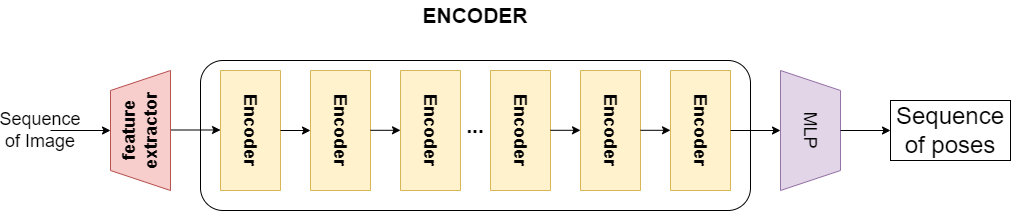
\includegraphics[width=\textwidth]{images/4_1_encoder_only}
    \caption{Encoder-only transformer}\label{fig:figure-encoder-only-transformer}
\end{figure}

\subsection{Encoder-decoder}\label{subsec:encoder-decoder}

For the encoder-decoder, we used the same encoder of the previous section, and we added a decoder part, which takes the output of the encoder as \textit{memory}, and a learnable vector which are also trained.
In this version of the network, we tried the same configurations of the encoder-only model but the feature extractor ResNet50, because the network requires more memory than those available on GPU.
The structure of the network is shown in figure 4.2.
\begin{figure}[H]
    \centering
    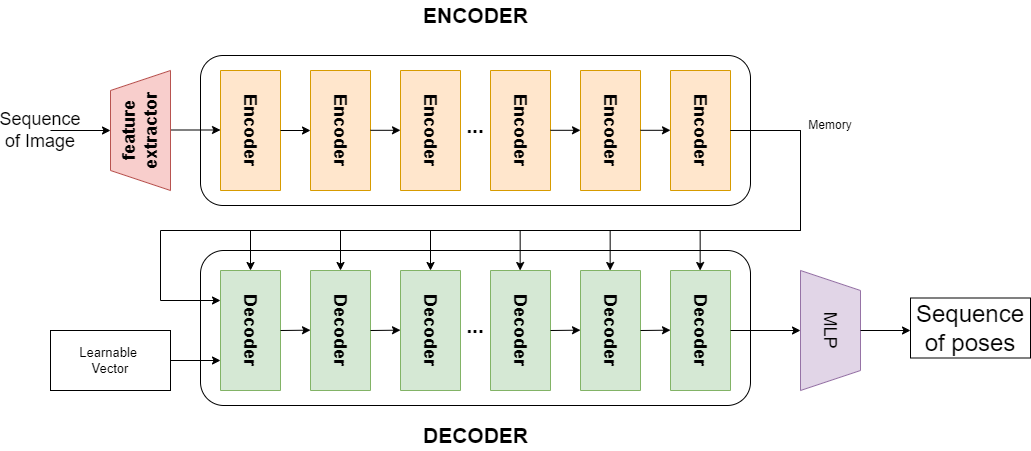
\includegraphics[width=\textwidth]{images/4_1_encoder_decoder}
    \caption{Encoder-Decoder transformer}\label{fig:figure-encoder-decoder-transformer}
\end{figure}

\subsection{Encoder-Decoder with auto-encoder}\label{subsec:encoder-decoder-with-auto-encoder}
In this version of the model, we used the same encoder-decoder model of the previous section, but we added a pose auto-encoder, which given the ground-truth of the pose, it increases the dimensionality of the input to 512 or 2048 and back to the original dimensionality.
The auto-encoder is split into two parts: first part brings the dimensionality from $x$ to 512 and 2048, the second part brings the dimensionality back to $x$, with $x$ depending on the representation format (6 for euler angles, and 12 for roto-translation matrix).
\begin{figure}[H]
    \centering
    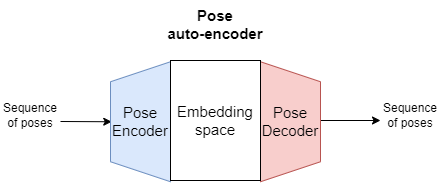
\includegraphics[width=0.5\textwidth]{images/4_1_pose_encoder}
    \caption{Pose auto-encoder}\label{fig:figure-pose-encoder}
\end{figure}

In the Figure 4.3, we can see how the auto-encoder is split in two parts.

We used the first part to create the ground-truth embedding of the pose, the second part to get the prediction of the pose from 512 or 2048 dimensionality.
So, the final structure of the model is shown in Figure 4.4.
\begin{figure}[H]
    \centering
    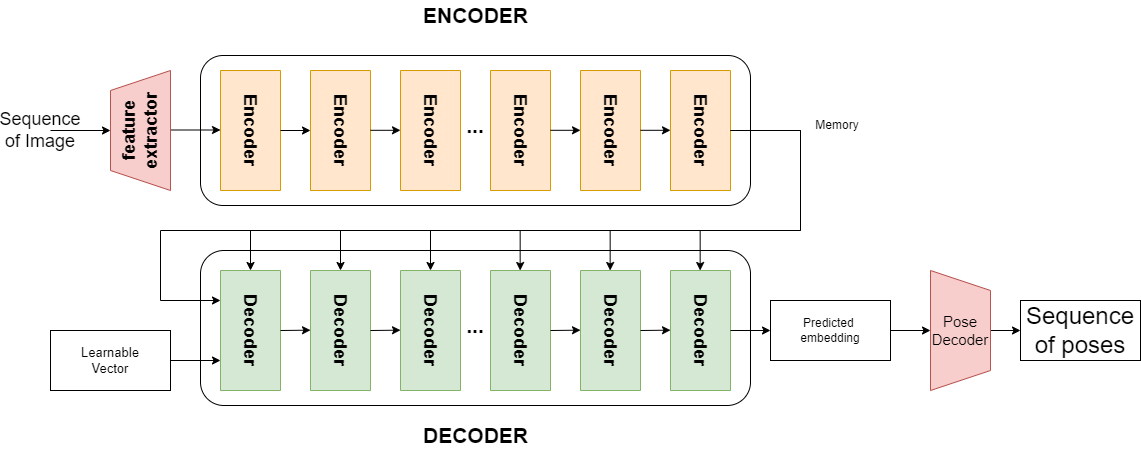
\includegraphics[width=\textwidth]{images/4_1_encoder_decoder_with_pose_autoencoder}
    \caption{Encoder-Decoder with pose auto-encoder}\label{fig:figure-encoder-decoder-with-pose-encoder}
\end{figure}

\subsection{Encoder-Decoder in autoregressive mode}\label{subsec:encoder-decoder-in-autoregressive-mode}
In this model, we replaced the parameter vector \textit{memory} with the output of the first part of the pose auto-encoder because the output is used to generate the ground-truth embedding used as target embedding, and the second part, as usual, is used to calculate the pose from embedding.

\begin{figure}[H]
    \centering
    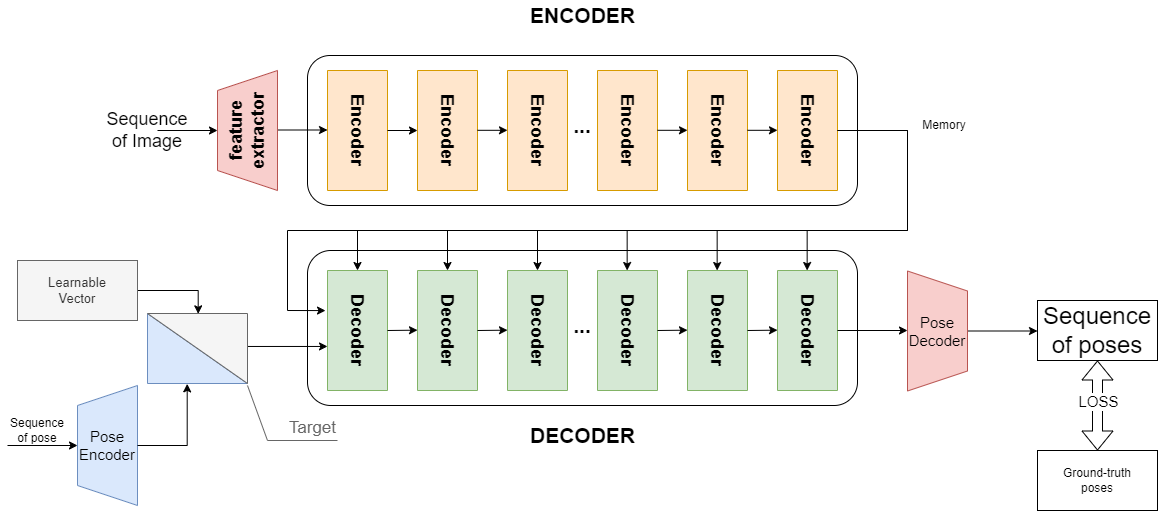
\includegraphics[width=\textwidth]{images/4_1_ar_train}
    \caption{Auto-regressive mode: training time.}\label{fig:figure-auto-regressive-train}
\end{figure}

In the figure 4.5, we can see the architecture of this model at \textbf{training time}, where the memory comes from the encoder, then, we construct the target by using the learnable vector as the upper-triangle of the target, and the embedding of the ground-truth as the lower-triangle of the target.
For the \textbf{inference time}, where we need to predict the pose one by one, starting from the second pose because the first one is the origin, in the figure 4.6, we can see the workflow of the model.
At first step of prediction, where we have to predict the second pose, we use the target which is composed like: $[origin\_emb, learnable\_vector[1\colon-1]]$ , for next step,
we will use: $[origin\_emb, first\_prediction, learnable\_vector[2\colon-1]]$, then $[origin\_emb, first\_prediction, second\_prediction, learnable\_vector[3\colon-1]]$, and so on so forth.
Meanwhile, the memory is not changed.

\begin{figure}[H]
    \centering
    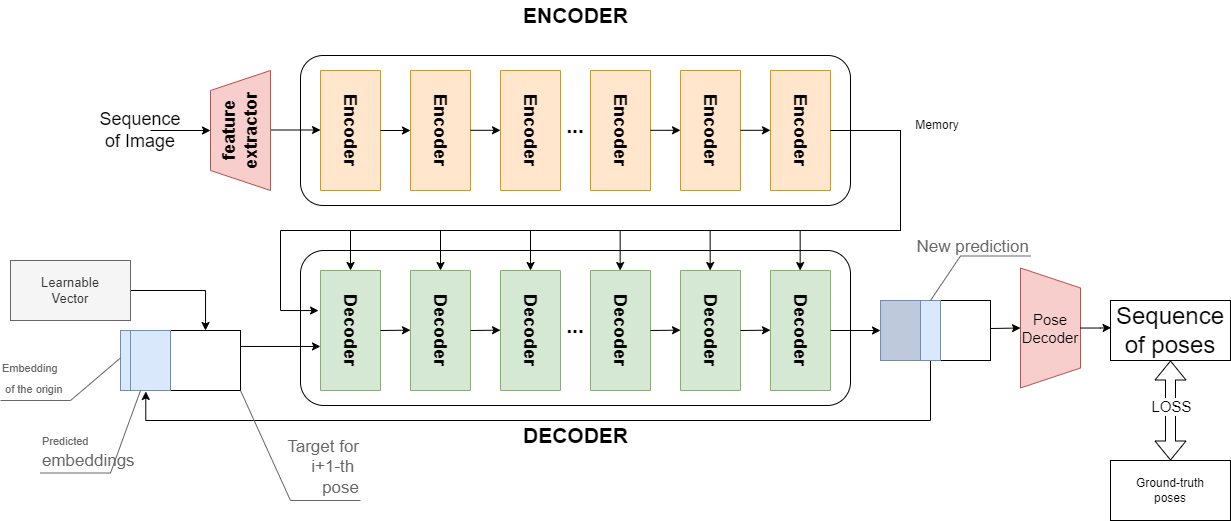
\includegraphics[width=\textwidth]{images/4_1_ar_inference}
    \caption{Autoregressive mode: inference time}\label{fig:figure-auto-regressive-inference}
\end{figure}
